\chapter{Implementation}
This chapter will focus on the implementation of various methods for generating a discrete distance field. It will start
with a basic brute-force approach before delving into optimizations and other algorithms. Each implementation will
include a short performance test for comparison between different implementations.

\section{Brute-force Approach}
A brute-force implementation for calculating the discrete distance field given a voxel grid is the most straight-forward
to implement but will suffer from performance; especially as world sizes get larger.

To compute the distance field for a voxel grid using a brute-force approach, we consider a voxel, \(V\) at
\((x, y, z)\). The algorithm starts iterating from the origin of the world \((0, 0, 0)\) and progresses incrementally
along each axis of the grid. For every voxel in the grid, the Manhattan distance is calculated to \(V\). This exhaustive
method, while producing an accurate distance field, must explore every other possible coordinate within the grid; this
can be seen in Algorithm~\ref{alg:brute_force}.

In the worst-case scenario, the algorithm must evaluate the distance for all \(N^3\), where \(N\) is the size of one
axis and the grid has uniform dimensions. Thus, the worst-case complexity is \(O(N^3)\). In the best-case, when the
voxel \(V\) is located near the origin a complexity of \(O(1)\) can be achieved, but this is highly unlikely.

\begin{algorithm}
    \caption{Brute Force Distance Field Calculation}
    \label{alg:brute_force}
    \begin{algorithmic}[1]
        \REQUIRE Voxel grid size \(N\), Voxel grid \(V\), Voxel location \((x, y, z)\)
        \ENSURE Distance field grid \(D\)
        \STATE Initialize \(D[i][j][k] \gets N\) for all \(i, j, k \in [0, N-1]\)
        \FOR{\(i = 0\) to \(N-1\)}
        \FOR{\(j = 0\) to \(N-1\)}
        \FOR{\(k = 0\) to \(N-1\)}
        \IF{\(V[i][j][k]\) is solid}
        \STATE \(d \gets |i - x| + |j - y| + |x - z|\) \COMMENT{Manhattan distance calculation, this will be common to
            all implementations.}
        \IF{\(d < D[i][j][k]\)}
        \STATE \(D[i][j][k] \gets d\) \COMMENT{Write only the shortest distance to the output.}
        \ENDIF
        \ENDIF
        \ENDFOR
        \ENDFOR
        \ENDFOR
        \STATE \textbf{Return:} \(D\)
    \end{algorithmic}
\end{algorithm}

\subsection{Performance Results}
At very small world sizes, the performance of the brute-force algorithm is sufficient; however the performance gets
exponentially worse the larger the world becomes, this can be seen in the FPS of the application in
Table~\ref{tab:brute_force_fps}. At a world size above \(256^3\), the amount of work required by each warp on the GPU
becomes too large resulting in the application crashing, as such the testing for this only went to a world size of
\(128^3\).

\begin{table}[h]
    \centering
    \sisetup{
        table-format=3.3,
        round-mode=places,
        round-precision=3
    }
    \vspace{0.5em}
    \begin{tabular}{l|*{5}{c}}
        \toprule
        \textbf{World Size} & \textbf{\(8^3\)} & \textbf{\(16^3\)} & \textbf{\(32^3\)} & \textbf{\(64^3\)} & \textbf{\(128^3\)} \\
        \midrule
        \textbf{Avg. FPS}   & 142.33702        & 142.335887        & 91.44403          & 2.30128           & 0.04184            \\
        \bottomrule
    \end{tabular}
    \caption{Frame rate of the brute-force algorithm at varying world sizes with a modification every 200ms.}
    \label{tab:brute_force_fps}
\end{table}

\begin{table}[h]
    \centering
    \sisetup{
        table-format=3.3,
        round-mode=places,
        round-precision=3
    }
    \vspace{0.5em}
    \resizebox{\textwidth}{!}{%
        \begin{tabular}{l|*{5}{c}}
            \toprule
            \textbf{World Size}               & \textbf{\(8^3\)}         & \textbf{\(16^3\)}      & \textbf{\(32^3\)}    & \textbf{\(64^3\)}    & \textbf{\(128^3\)}     \\
            \midrule
            \textbf{Avg. Time (ms)}           & 0.13085426               & 0.72909933             & 8.415086             & 431.46756            & 25854.305              \\
            \textbf{Std. Deviation (ms)}      & 0.07906039               & 0.72129595             & 0.6034345            & 23.69193             & 43.82031               \\
            \textbf{Confidence Interval (ms)} & (0.12865908, 0.13304944) & (0.7251273, 0.7330714) & (8.400318, 8.429853) & (428.5129, R34.4222) & (25830.484, 25878.125) \\
            \bottomrule
        \end{tabular}
    }
    \caption{Distance field compute shader execution time using the brute-force algorithm.}
    \label{tab:brute_force}
\end{table}

The results in Table~\ref{tab:brute_force} highlight how a brute-force approach is unsuitable for large dynamic worlds.
A common optimization is chunking to split a large world into smaller ``chunks'' as described in
Section~\ref{sec:chunking}.

\section{Splitting a World into Chunks} \label{sec:chunking}
Partitioning, or chunking, is a common approach to divide a large problem into smaller manageable problems. In the
context of voxels world, sparse voxel octrees (SVO) are an approach for dividing a large dense representation of a voxel
grid into a more sparse format with data only stored where it's needed; this makes it more efficient to process and
render~\cite{laine2010efficient,mileff2019simplified,van2015real}.

Given that a brute-force approach has acceptable performance at a world size of \(16^3\), as can be seen in Table
\ref{tab:brute_force}, we can divide the whole world into smaller \(16^3\) chunks. This will allow for updates in one
chunk to be localized, as such updates will not be required to update the whole world reducing the amount of iterations
required to update a distance field.

For a \(512^3\) sized world, we could divide it into \(32,768\) chunks each with a size of \(16^3\). A worst-case
complexity for this significantly larger world is now \(O(16^3)\) compared to the \(O(512^3)\) it would otherwise be
without a chunking approach.

Chunks, however, present a significant problem in distance field generation as they can introduce inaccuracies between
chunk borders. This can happen if we don't consider the voxels in an adjacent chunk when calculating distances, there
are three potential solutions to this problem:

\begin{enumerate}
    \item When iterating over a chunk, iterate over a size \(X + 2, Y + 2, Z + 2\) to introduce ``padding''. Checking
          neighbours that are in padding region will be treated as solid which will introduce a border in the distance field
          that would force rays to march into the beginning of the next chunk.
    \item Include the adjacent chunks as input to the distance field compute shader. Out-of-bounds accesses should
          result in checking neigbouring chunks; however, this expands the number of voxels needed to be checked and will
          still suffer from inaccuracies if the nearest solid voxel is not in a neighbouring chunk.
    \item Combining the first approach, with multiple passes. An initial distance field calculation is computed for each
          chunk independently. To ensure accurate distances at chunk boundaries, another pass through the world can be done
          that includes neighbour information. Multiple, more global, passes will ensure distances eventually converge on the
          correct distance value~\cite{gorobets2023approach,sinharoy1993finding,xu2015fast}.
\end{enumerate}

\subsection{Padding}
The chosen approach at this point, is to introduce padding to an individual chunk when calculating the distance field.
With this approach the worst-case complexity is slightly worse than without using chunking. Without chunks a \(16^3\)
world, has a complexity \(O(N^3)\), with chunks we require padding and so a chunk of the same size would have a
complexity of \(O((N + 2)^3)\).

To account for the ``padding'' around a chunk, out-of-bounds accesses will be treated as a solid voxel.

\begin{algorithm}[H]
    \caption{Get Voxel at \((x, y, z)\)}
    \label{alg:get_voxel}
    \begin{algorithmic}[1]
        \REQUIRE Voxel grid \(V\), position \(x, y, z\)
        \IF{\(x, y, z\) is within bounds of \(V\)}
        \RETURN \(V[x][y][z]\)
        \ELSE
        \RETURN Solid voxel
        \ENDIF
    \end{algorithmic}
\end{algorithm}

The algorithm for the distance field calculation remains largely unchanged except for now using Algorithm
\ref{alg:get_voxel} to access the voxel grid \(V\) instead of direct access. The updated algorithm is now implemented
as follows.

\begin{algorithm}[H]
    \caption{Brute force Distance Field Calculation (With chunks)}
    \begin{algorithmic}[1]
        \REQUIRE Voxel grid size \(N\), Voxel grid \(V\), Voxel location \((x, y, z)\)
        \ENSURE Distance field grid \(D\)
        \STATE Initialize \(D[i][j][k] \gets N\) for all \(i, j, k \in [0, N-1]\)
        \FOR{\(i = -1\) to \(N\)}
        \FOR{\(j = -1\) to \(N\)}
        \FOR{\(k = -1\) to \(N\)}
        \STATE \texttt{voxel} $\gets$ \texttt{Get Voxel at} \((i, j, k)\)
        \IF{\texttt{voxel is solid}}
        \STATE \(d \gets |i - x| + |j - y| + |x - z|\)
        \IF{\(d < D[i][j][k]\)}
        \STATE \(D[i][j][k] \gets d\)
        \ENDIF
        \ENDIF
        \ENDFOR
        \ENDFOR
        \ENDFOR
        \STATE \textbf{Return:} \(D\)
    \end{algorithmic}
\end{algorithm}

\subsection{Performance Results}
Based on the performance results of the brute-force approach, as can be seen in Table~\ref{tab:brute_force}, the
proceeding tests will use a chunk size of \(16^3\). The key improvement in using chunks is that the total world size is
theoretically only limited by the memory consumption, and number of storage buffers supported by the GPU. Sufficiently
large updates spanning multiple chunks will be less performant, but we can expect that a small localized update
affecting only a couple of chunks will have only marginally worse performance than the previous approach.

We can see from the performance results in Table~\ref{tab:chunks_perf} that we are able to maintain a low average
execution time when updating the distance field; however, FPS gets significantly worse at larger world sizes, this is
due to the cost of managing a high amount of storage buffer objects and memory read/write operations.

\begin{table}[h!]
    \centering
    \sisetup{
        table-format=3.3,
        round-mode=places,
        round-precision=3
    }
    \vspace{0.5em}
    \begin{tabular}{l|*{5}{c}}
        \toprule
        \textbf{World Size}          & \textbf{\(32^3\)} & \textbf{\(64^3\)} & \textbf{\(128^3\)} & \textbf{\(256^3\)} & \textbf{\(512^3\)} \\
        \midrule
        \textbf{Avg. FPS}            & 141.02969         & 140.32344         & 88.75602           & 22.13375           & 3.37203            \\
        \textbf{Avg. Execution Time} & 0.8090571         & 0.7992149         & 0.7797105          & 0.7632012          & 0.7504562          \\
        \textbf{\% Improvement}      & 54.2251\%         & 5997.63\%         & 212032\%           & Inf\%              & Inf\%              \\
        \bottomrule
    \end{tabular}
    \caption{Frame rate, and execution time, of the brute-force algorithm, when using a chunk size of \(16^3\), at
        varying world sizes with a modification to the world every 200ms. Percentage improvement is the improvement in
        frame rate compared to a comparably sized world without chunks, as demonstrated in Table~\ref{tab:brute_force_fps}.}
    \label{tab:chunks_perf}
\end{table}

\FloatBarrier

\section{Fast Iterative Method} \label{sec:fim}
The fast marching method (FMM)~\cite{sethian1999fast} and fast iterative method (FIM)~\ref{jeong2008fast} are
approaches used for solving a boundary value problem; in the case of a voxel grid distance field our boundary problem is
defined as identifying the distances for each air voxel to the nearest voxel. FMM is a sequential algorithm that relies
on processing scans of the grid in the correct order and complex data structures making it unsuitable for the GPU; FIM
is an enhancement that doesn't have those same requirements but can achieve the same result.

FIM computes distance fields by propagating distance information outward from known boundary regions; the boundary
region for a voxel grid is computed by setting all solid voxels to a distance of 0 and all air voxels to a sufficiently
large number, this can be seen in Figure~\ref{fig:fim_init} and Algorithm~\ref{alg:fim_init}.

\begin{figure}[htbp]
    \centering
    \begin{subfigure}[t]{0.32\textwidth}
        \centering
        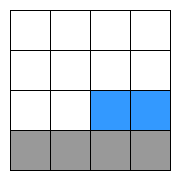
\includegraphics[width=\textwidth]{figures/voxel_grid.drawio.png}
        \caption{A 2D representation of the world. Empty voxels are indicated by white cells.}
    \end{subfigure}
    \hfill
    \begin{subfigure}[t]{0.32\textwidth}
        \centering
        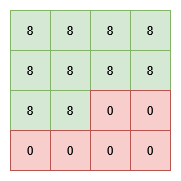
\includegraphics[width=\textwidth]{figures/voxel_grid_fmm_init.drawio.png}
        \caption{A 2D representation of a voxel grid initialized in preparation for FIM.}
    \end{subfigure}
    \caption{The corresponding initialized distance field for a voxel grid.}
    \label{fig:fim_init}
\end{figure}

On a GPU, each voxel can be processed in parallel by leveraging atomic minimums. When distance information is propagated
in a single iteration only the minimum value is saved to the distance field. A distance can at most propagate 1 voxel
away from the voxel being processed, this means that to achieve an accurate distance field FIM must be executed on the
distance field several times until shortest distances have been calculated for all voxels, the effect of several
iterations can be seen in Figure~\ref{fig:fim_convergence}.

\begin{figure}[htbp]
    \centering
    \begin{subfigure}[t]{0.24\textwidth}
        \centering
        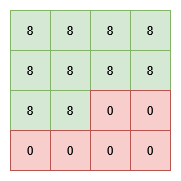
\includegraphics[width=\textwidth]{figures/voxel_grid_fmm_init.drawio.png}
        \caption{Iteration 0.}
    \end{subfigure}
    \hfill
    \begin{subfigure}[t]{0.24\textwidth}
        \centering
        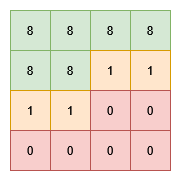
\includegraphics[width=\textwidth]{figures/voxel_grid_fmm_1.drawio.png}
        \caption{Iteration 1.}
    \end{subfigure}
    \hfill
    \begin{subfigure}[t]{0.24\textwidth}
        \centering
        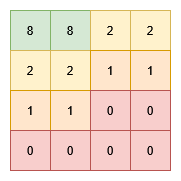
\includegraphics[width=\textwidth]{figures/voxel_grid_fmm_2.drawio.png}
        \caption{Iteration 2.}
    \end{subfigure}
    \hfill
    \begin{subfigure}[t]{0.24\textwidth}
        \centering
        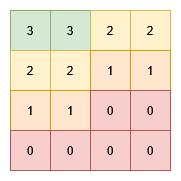
\includegraphics[width=\textwidth]{figures/voxel_grid_fmm_3.drawio.png}
        \caption{Iteration 3.}
    \end{subfigure}
    \caption{Convergence of distance field values after several iterations when using FIM.}
    \label{fig:fim_convergence}
\end{figure}

The number of iterations required for convergence is proportional to the size of a chunk - a voxel that is \(N\) units
away from the chunk boundary, will require at least \(N\) units to receive the correct distance value. As such, given a
chunk of size \(C = 8\), the total number of voxels to process is \(N = 8^3\), the worst-case computation will be
\(O(8N)\).

Convergence can be handled on the CPU or on the GPU, the chosen approach was to implement a single iteration of the FIM
algorithm, as can be seen in Algorithm~\ref{alg:fim}, as a compute shader. The CPU will dispatch the compute shader
until no changes have been made to the distance field, as such it can be concluded that distances have converged.

\begin{algorithm}[H]
    \caption{Fast Iterative Method, Distance Field Initialization}
    \label{alg:fim_init}
    \begin{algorithmic}[1]
        \REQUIRE Voxel grid size \(N\), Voxel grid \(V\), Voxel location \((x, y, z)\)
        \ENSURE Distance field grid \(D\)
        \STATE \texttt{voxel} $\gets$ \texttt{Get Voxel at} \((x, y, z)\)
        \IF{\texttt{voxel is solid}}
        \STATE \(D[x][y][z] \gets 0\)
        \ELSE
        \STATE \(D[x][y][z] \gets N * 2\)
        \ENDIF
    \end{algorithmic}
\end{algorithm}

\begin{algorithm}[H]
    \caption{Fast Iterative Method}
    \label{alg:fim}
    \begin{algorithmic}[1]
        \REQUIRE Voxel grid size \(N\), Voxel grid \(V\), Voxel location \((x, y, z)\)
        \ENSURE Distance field grid \(D\)
        \STATE \texttt{voxel} $\gets$ \texttt{Get Voxel at} \((x, y, z)\)
        \IF{\texttt{voxel is solid}}
        \STATE \textbf{Return:} \(D\)
        \ENDIF

        \STATE Initialize $d_{min} \gets N * 2$
        \FOR{neighbours $n$ of voxel}
        \STATE \texttt{neighbour} $\gets$ \texttt{Get Voxel at} $n$
        \IF{\texttt{neighbour is solid}}
        \STATE $d_n \gets 0$
        \ELSE
        \STATE $d_n \gets$ distance value at $n$
        \ENDIF
        \STATE $d_n \gets d_n + 1$
        \STATE $d_{min} \gets \min(d_{min}, d_n)$
        \ENDFOR

        \IF{$d_{min} <$ current distance of $voxel$}
        \STATE Update $D$ at $(x, y, z)$ to $d_{min}$
        \STATE Mark distance field as changed
        \ENDIF
        \STATE \textbf{Return:} \(D\)
    \end{algorithmic}
\end{algorithm}

\subsection{Performance Results}
FIM is expected to be significantly more efficient than the brute-force approach, as such the optimal chunk size to use
needs to be determined first. We can see from Table~\ref{tab:fim_chunks}, that we are able to compute the distance field
for a chunk much faster; however at $128^3$ sized chunks the variance in the number of iterations required for
convergence leads to inconsistent performance.

\begin{table}[h]
    \centering
    \sisetup{
        table-format=3.3,
        round-mode=places,
        round-precision=3
    }
    \vspace{0.5em}
    \resizebox{\textwidth}{!}{%
        \begin{tabular}{l|*{5}{c}}
            \toprule
            \textbf{Chunk Size}                         & \textbf{\(8^3\)} & \textbf{\(16^3\)} & \textbf{\(32^3\)} & \textbf{\(64^3\)} & \textbf{\(128^3\)} \\
            \midrule
            \textbf{Total Avg. Time (ms)}               & 0.0408411        & 0.05089584        & 0.1566725         & 1.089782          & 17.556416          \\
            \textbf{Std. Deviation (ms)}                & 0.012230597      & 0.009375835       & 0.07214462        & 0.5198319         & 16.088636          \\
            \textbf{Average Iterations for Convergence} & 1.0313779        & 1.1514729         & 1.4801816         & 2.3467271         & 6.194286           \\
            \bottomrule
        \end{tabular}
    }
    \caption{Distance field compute shader execution time (as a total of all iterations required to achieve convergence)
        using the FIM algorithm.}
    \label{tab:fim_chunks}
\end{table}

There is a substantial increase in performance for distance field computation of single chunks; however, the cost of
CPU-GPU synchronization means that once there are several chunks that need updating there is a significant amount of
time spent on waiting for various fences to be signalled for synchronization. The time spent waiting for fences is time
not spent doing useful work on the GPU nor CPU, as such we can observe a decline in performance at large world sizes
with several chunks as can be seen in Figure~\ref{fig:fim_perf}.

\begin{figure}
    \centering
    \begin{tikzpicture}
        \begin{groupplot}[
                group style={
                        group size=1 by 2,
                        vertical sep=4cm,
                    },
                grid=major
            ]

            \nextgroupplot[
                title={Frame Performance},
                xlabel={World Size (voxels)}, ylabel={Average FPS},
                xtick={64,128,256,512,1024},
                xticklabel style={rotate=45},
                legend pos=outer north east
            ]
            \addplot[red, thick, mark=*] coordinates {
                    (64,95.30249) (128,75.96144) (256,34.19493) (512,3.57249)
                };
            \addlegendentry{$16^3$ Chunks}

            \addplot[green, thick, mark=*] coordinates {
                    (64,95.03077) (128,83.51576) (256,45.91034) (512,21.19063) (1024,3.228742)
                };
            \addlegendentry{$32^3$ Chunks}

            \addplot[blue, thick, mark=*] coordinates {
                    (64,68.15260) (128,46.48674) (256,23.07958) (512,14.77858) (1024,4.26064)
                };
            \addlegendentry{$64^3$ Chunks}

            \nextgroupplot[
                title={Distance Field Computation},
                xlabel={World Size (voxels)}, ylabel={Avg. Execution Time (ms)},
                xtick={64,128,256,512,1024},
                xticklabel style={rotate=45},
                legend pos=outer north east
            ]
            \addplot[red, thick, mark=*] coordinates {
                    (64,0.07576919) (128,0.103998095) (256,0.22743346) (512,0.4117954)
                };
            \addlegendentry{$16^3$ Chunks}

            \addplot[green, thick, mark=*] coordinates {
                    (64,0.19434363) (128,0.32839835) (256,0.5721531) (512,0.81162566) (1024,1.0872366)
                };
            \addlegendentry{$32^3$ Chunks}

            \addplot[blue, thick, mark=*] coordinates {
                    (64,1.245831) (128,1.941034) (256,5.226551) (512,7.010742) (1024,7.7111363)
                };
            \addlegendentry{$64^3$ Chunks}
        \end{groupplot}
    \end{tikzpicture}

    \caption{Comparison of the performance of the Fast Iterative Method at different world and chunk sizes.}
    \label{fig:fim_perf}
\end{figure}

\section{Jump Flooding Algorithm} \label{sec:jfa}
The Jump Flooding Algorithm (JFA) works by propagating information about the closest occupied voxels through a grid
using a pattern of ``jumps'' with progressively decreasing step sizes. Unlike traditional flooding algorithms that work
with neighboring cells, JFA allows information to ``jump'' across larger distances initially, making it highly efficient.

For a distance field from a voxel occupancy grid, this can be seen in Figure~\ref{fig:jfa_passes} and
Algorithm~\ref{alg:jfa}:
\begin{enumerate}
    \item Initialize the distance field with an initial known boundary, similar to the initialized required for FIM as
          seen in Figure~\ref{fig:fim_init}.
    \item Execute multiple passes with decreasing step sizes using powers of 2.
    \item In each pass, the shortest distances are gathered from neighbouring voxels using the step size.
\end{enumerate}

\begin{figure}[htbp]
    \centering
    \begin{subfigure}[t]{0.32\textwidth}
        \centering
        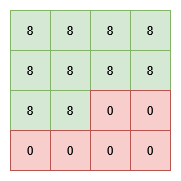
\includegraphics[width=\textwidth]{figures/voxel_grid_fmm_init.drawio.png}
        \caption{Initialized distance field.}
    \end{subfigure}
    \hfill
    \begin{subfigure}[t]{0.32\textwidth}
        \centering
        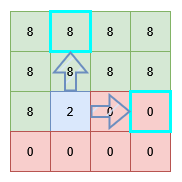
\includegraphics[width=\textwidth]{figures/jfa_pass_1.drawio.png}
        \caption{Pass 1, Step Size 2.}
    \end{subfigure}
    \hfill
    \begin{subfigure}[t]{0.32\textwidth}
        \centering
        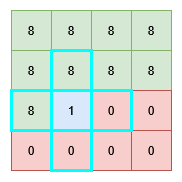
\includegraphics[width=\textwidth]{figures/jfa_pass_2.drawio.png}
        \caption{Pass 2, Step Size 1}
    \end{subfigure}
    \caption{Illustration of checking neighbours at decreasing step sizes.}
    \label{fig:jfa_passes}
\end{figure}


JFA operates in \(log(N)\) passes for an \(NxN\) grid, with the step size halving in each pass - starting with a step
size \(N / 2\) decreasing to a step size of \(1\) using powers of 2. The expected complexity of JFA is \(O(N^3log(N))\).
JFA is a highly efficient algorithm; however, due to the nature of ``jumps'' and ambiguous closest point information it
is possible for the true shortest distances to not be chosen when checking neighbouring voxels, this can result in a
distance field that is not exact.

Jump Flooding requires multiple passes for distance information to be propagated through the entire distance field - the
chosen approach is for the compute shader to implement a single iteration of JFA, as seen in Algorithm~\ref{alg:jfa}.
The CPU will be responsible for dispatching the compute shader at decreasing step sizes until a step size of 1 is
reached. This will again introduce CPU-GPU synchronization losses but makes implementing the algorithm simpler. Similar
to FIM, it is required that the distance field is initialized with large values for air voxels, and distances of \(0\)
for solid voxels as seen in Algorithm~\ref{alg:fim_init}.

Since information needs to be written to, and read from, the distance field at the same time it is necessary to employ
a ``ping-pong'' buffer approach where buffer A is only used to read distance information, while new distance information
is written to buffer B - these buffers are then swapped before the next iteration of JFA. This will eliminate any race
conditions that may arise.

\begin{algorithm}[H]
    \caption{Jump Flooding Algorithm}
    \label{alg:jfa}
    \begin{algorithmic}[1]
        \REQUIRE Voxel grid size \(N\), Voxel grid \(V\), Voxel location \((x, y, z)\), Step Size \(S\)
        \ENSURE Distance field grid \(D\)
        \STATE \texttt{voxel} $\gets$ \texttt{Get Voxel at} \((x, y, z)\)
        \IF{\texttt{voxel is solid}}
        \STATE \textbf{Return:} \(D\)
        \ENDIF

        \STATE Initialize $d_{min} \gets$ distance value of voxel at \((x, y, z)\)
        \FOR{neighbours $n$ of voxel $S$ steps away}
        \STATE \texttt{neighbour} $\gets$ \texttt{Get Voxel at} $n$
        \STATE $d_{n} \gets$ distance value of voxel at $neighbour$
        \STATE $d_{min} \gets \min(d_{min}, d_n + S)$
        \ENDFOR
        \STATE \textbf{Return:} \(D\)
    \end{algorithmic}
\end{algorithm}

\subsection{Performance Results}
We can see from Table~\ref{tab:jfa_perf} and Figure~\ref{fig:jfa_perf_2} that the compute shader execution time, as a
total of all dispatches required to complete JFA for a single chunk, is significantly quicker that FIM; it is feasible
to now use chunks as big as \(64^3\). This improved performance is not entirely comparable to FIM, as JFA only produces
an approximate distance field, this means that the render of the distance field will contain minor artifacts where
distances don't align with the true surface which can be seen in Figure~\ref{fig:fim_jfa_comp}.

\begin{table}[h]
    \centering
    \sisetup{
        table-format=3.3,
        round-mode=places,
        round-precision=3
    }
    \vspace{0.5em}
    \resizebox{\textwidth}{!}{%
        \begin{tabular}{l|*{5}{c}}
            \toprule
            \textbf{Chunk Size}           & \textbf{\(8^3\)} & \textbf{\(16^3\)} & \textbf{\(32^3\)} & \textbf{\(64^3\)} & \textbf{\(128^3\)} \\
            \midrule
            \textbf{Total Avg. Time (ms)} & 0.031079482      & 0.37563447        & 0.07390518        & 0.38933817        & 8.052377           \\
            \textbf{Std. Deviation (ms)}  & 0.0060166107     & 0.0011396826      & 0.014052732       & 0.1003621         & 3.9264889          \\
            \bottomrule
        \end{tabular}
    }
    \caption{Distance field compute shader execution time using the JFA algorithm.}
    \label{tab:jfa_perf}
\end{table}

\begin{figure}[htbp]
    \centering
    \begin{subfigure}[t]{0.49\textwidth}
        \centering
        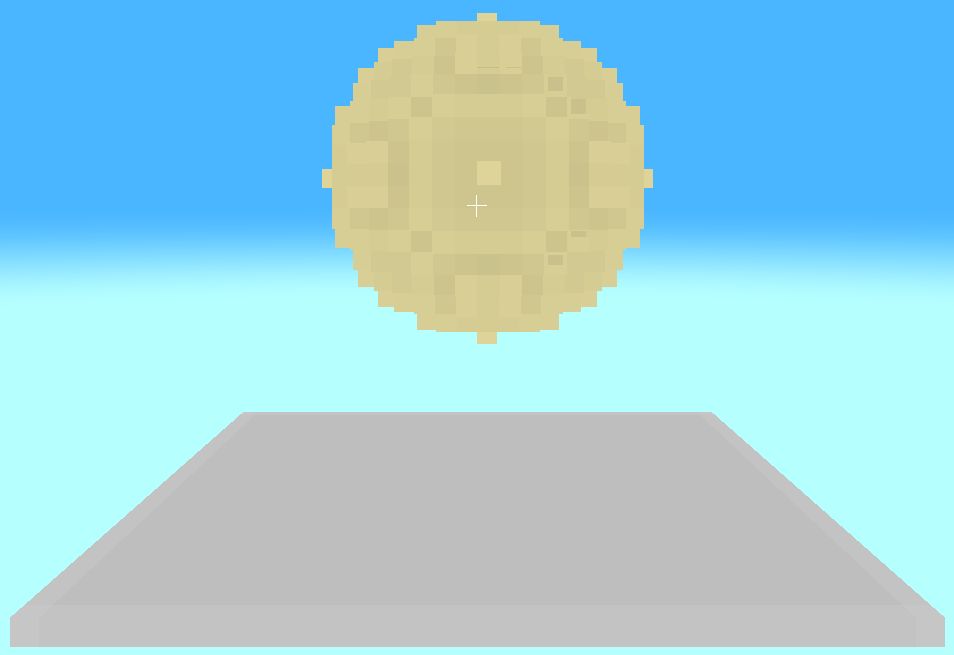
\includegraphics[width=\textwidth]{figures/demo_fim.png}
        \caption{Fast Iterative Method}
    \end{subfigure}
    \hfill
    \begin{subfigure}[t]{0.49\textwidth}
        \centering
        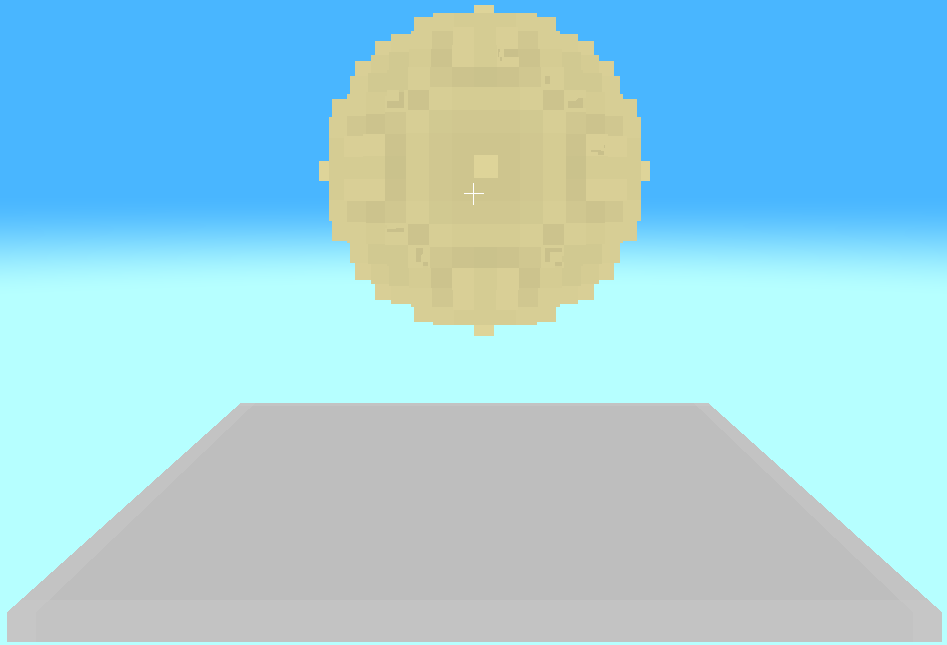
\includegraphics[width=\textwidth]{figures/demo_jfa.png}
        \caption{Jump Flooding Algorithm}
    \end{subfigure}
    \caption{Comparison of rendering an exact and approximate distance field.}
    \label{fig:fim_jfa_comp}
\end{figure}

\begin{figure}
    \centering
    \begin{tikzpicture}
        \begin{groupplot}[
                group style={
                        group size=1 by 2,
                        vertical sep=4cm,
                    },
                grid=major
            ]

            \nextgroupplot[
                title={Frame Performance},
                xlabel={World Size (voxels)}, ylabel={Average FPS},
                xtick={64,128,256,512,1024},
                xticklabel style={rotate=45},
                legend pos=outer north east
            ]
            \addplot[red, thick, mark=*] coordinates {
                    (64,140.95991) (128,139.21750) (256,58.62559) (512,7.22179)
                };
            \addlegendentry{$16^3$ Chunks}

            \addplot[green, thick, mark=*] coordinates {
                    (64,140.72791) (128,132.19121) (256,97.06799) (512,48.7238) (1024,5.75885)
                };
            \addlegendentry{$32^3$ Chunks}

            \addplot[blue, thick, mark=*] coordinates {
                    (64,79.47583) (128,59.17962) (256,52.03550) (512,43.55900) (1024,28.47231)
                };
            \addlegendentry{$64^3$ Chunks}

            \nextgroupplot[
                title={Distance Field Computation},
                xlabel={World Size (voxels)}, ylabel={Avg. Execution Time (ms)},
                xtick={64,128,256,512,1024},
                xticklabel style={rotate=45},
                legend pos=outer north east
            ]
            \addplot[red, thick, mark=*] coordinates {
                    (64,0.029005498) (128,0.025463749) (256,0.037660573) (512,0.045116894)
                };
            \addlegendentry{$16^3$ Chunks}

            \addplot[green, thick, mark=*] coordinates {
                    (64,0.06540906) (128,0.06330304) (256,0.066737905) (512,0.079189345) (1024,0.113251306)
                };
            \addlegendentry{$32^3$ Chunks}

            \addplot[blue, thick, mark=*] coordinates {
                    (64,0.38292697) (128,0.367488) (256,0.3376916) (512,0.3192967) (1024,0.31650382)
                };
            \addlegendentry{$64^3$ Chunks}
        \end{groupplot}
    \end{tikzpicture}
    \caption{Comparison of the performance of the Jump Flooding Algorithm at different world and chunk sizes.}
    \label{fig:jfa_perf_2}
\end{figure}

\section{Coarse JFA with FIM Refinement} \label{sec:hybrid_jfa_fim}
We observed that JFA can produce an approximate distance field, with minimal artifacts, very quickly in
Section~\ref{sec:jfa}. FIM is efficient at producing an accurate distance field but the distribution in the number of
iterations required for convergence can have a negative impact on the performance; as described in
Section~\ref{sec:fim}, FIM works by propagating minimum distances through the distance field.

It is possible to use a combination of JFA and FIM to increase the execution speed, compared to a pure FIM
implementation, and maintain the computation on an exact distance field; the implementation for this uses the following
3 steps, with each step being defined in its own compute shader and being dispatched by the CPU in series:

\begin{enumerate}
    \item \textbf{Algorithm~\ref{alg:fim_init}}: to initialize the distance field.
    \item \textbf{Algorithm~\ref{alg:jfa}}: to create a more accurate ``seed'' that FIM can be run against to reduce the
          number of iterations required for FIM to converge on the correct distance values.
    \item \textbf{Algorithm~\ref{alg:fim}}: to converge distance values to their minimums.
\end{enumerate}

\subsection{Performance Results}
Executing the distance field compute shader on single chunks of varying sizes, as seen in
Table~\ref{tab:hybrid_jfa_fim_perf}, we observe that the number of required iterations to achieve convergence is
decreased compared to running FIM on a freshly initialized distance field as seen in Section~\ref{sec:fim}. The total
execution time is also less compared to pure FIM, especially as chunk sizes get larger.

\begin{table}[h]
    \centering
    \sisetup{
        table-format=3.3,
        round-mode=places,
        round-precision=3
    }
    \resizebox{\textwidth}{!}{%
        \begin{tabular}{l|*{5}{c}}
            \toprule
            \textbf{Chunk Size}                         & \textbf{\(8^3\)} & \textbf{\(16^3\)} & \textbf{\(32^3\)} & \textbf{\(64^3\)} & \textbf{\(128^3\)} \\
            \midrule
            \textbf{Total Avg. Time (ms)}               & 0.04326828       & 0.042948034       & 0.142226286       & 0.8856182         & 16.556087          \\
            \textbf{Std. Deviation (ms)}                & 0.014001529      & 0.0082087135      & 0.004889435       & 0.48032447        & 13.672007          \\
            \textbf{Average Iterations for Convergence} & 0.21335079       & 0.41733277        & 0.9516885         & 1.2535588         & 4.1610336          \\
            \bottomrule
        \end{tabular}
    }
    \caption{Distance field compute shader execution time using hybrid JFA and FIM approach. Compared against a pure
        FIM execution.}
    \label{tab:hybrid_jfa_fim_perf}
\end{table}

\section{Level-of-detail with JFA and FIM} \label{sec:lod_jfa_fim}
Using the previous hybrid JFA and FIM approach in Section~\ref{sec:hybrid_jfa_fim} optimized the execution of FIM;
however, we lost the advantage of excellent execution time that pure JFA results in as was visible in
Figure~\ref{fig:jfa_perf_2}.

We can reduce the amount of expensive work the GPU needs to do calculating exact distance fields only for the chunks
where it is necessary to have precise surface information. Chunks that are determined to be of less significance can
suffice with only JFA being run against them, this way they have a distance field representation that closely matches
the true surface and when rendered produce a passable result at a distance.

The approach in this section is similar to level-of-detail traditionally used in video games with mesh rendering, where
far away meshes are composed of fewer triangles to reduce the performance strain of that mesh as a large amount of
detail is not necessary for objects that will only take up a small amount of space in the displayed image.

Level-of-detail can be implemented for our approach by executing JFA for chunks that fall outside a ``focal point'',
and only executing FIM on chunks that are within the focal point. We can vary the amount of detail in the world overall
by increasing the focus size. The execution of FIM would be carried out on chunks that have already had JFA run on
them. An overall implementation of this can be seed in Algorithm~\ref{alg:jfa_fim_focus}, with the decision of what
algorithm to run being decided by the CPU, and the individual algorithms being implemented as their own compute shaders
executed by the GPU.

\begin{algorithm}[H]
    \caption{JFA and FIM with focus area}
    \label{alg:jfa_fim_focus}
    \begin{algorithmic}[1]
        \REQUIRE Chunk voxel grid \(C_{voxels}\), Chunk position \(C_{pos}\), Focus area \(F\), Focus size \(F_{size}\)
        \ENSURE Distance field grid \(D\)

        \STATE Initialize $F_{min} \gets F - F_{size}$
        \STATE Initialize $F_{max} \gets F + F_{size}$

        \STATE Execute \texttt{Algorithm~\ref{alg:fim_init}} on $C_{voxels}$
        \STATE Execute \texttt{Algorithm~\ref{alg:jfa}} on $C_{voxels}$

        \IF{$C_{pos} >= F_{min}$ and $C_{pos} <= F_{max}$}
        \STATE Execute \texttt{Algorithm~\ref{alg:fim}} on $C_{voxels}$
        \ENDIF
    \end{algorithmic}
\end{algorithm}

\subsection{Performance Results}
The focal point for all the following test was located at the center of the world; the effect of changing the focus size
was the focus. We observe from Figure~\ref{fig:lod_fps_perf} and Figure~\ref{fig:lod_comp_perf} that increasing the
focus size has a significant impact on the performance; however, as can be seen from
Figure~\ref{fig:focus_size_artifacts} there is a significant increase in visual fidelity as the focus size increases and
more chunks have an exact distance field computed using FIM.

\begin{figure}
    \centering
    \begin{tikzpicture}
        \begin{groupplot}[
                group style={
                        group size=2 by 2,
                        vertical sep=2cm,
                        horizontal sep=2cm,
                    },
                grid=major,
            ]

            \nextgroupplot[
                title={1x1 Focus Size},
                xlabel={World Size (voxels)}, ylabel={Average FPS},
                xtick={64,128,256,512,1024},
                xticklabel style={rotate=45},
                legend pos=north east
            ]
            \addplot[green, thick, mark=*] coordinates {
                    (64,160.51333) (128,152.31134) (256,103.35540) (512,49.47920) (1024,7.85048)
                };
            \addlegendentry{$32^3$ Chunks}

            \addplot[blue, thick, mark=*] coordinates {
                    (64,80.72423) (128,63.52796) (256,53.11886) (512,45.2700) (1024,28.71499)
                };
            \addlegendentry{$64^3$ Chunks}

            \nextgroupplot[
                title={2x2 Focus Size},
                xlabel={World Size (voxels)}, ylabel={Average FPS},
                xtick={64,128,256,512,1024},
                xticklabel style={rotate=45},
                legend pos=north east
            ]
            \addplot[green, thick, mark=*] coordinates {
                    (64,158.80035) (128,141.77115) (256,96.39616) (512,50.01648) (1024,7.58719)
                };
            \addlegendentry{$32^3$ Chunks}

            \addplot[blue, thick, mark=*] coordinates {
                    (64,83.71295) (128,52.001065) (256,38.56683) (512,37.65046) (1024,28.33969)
                };
            \addlegendentry{$64^3$ Chunks}

            \nextgroupplot[
                title={4x4 Focus Size},
                xlabel={World Size (voxels)}, ylabel={Average FPS},
                xtick={64,128,256,512,1024},
                xticklabel style={rotate=45},
                legend pos=north east,
            ]
            \addplot[green, thick, mark=*] coordinates {
                    (64,151.27016) (128,105.07455) (256,62.19417) (512,46.41498) (1024,7.3627)
                };
            \addlegendentry{$32^3$ Chunks}

            \addplot[blue, thick, mark=*] coordinates {
                    (64,83.74165) (128,50.44744) (256,26.73361) (512,21.67194) (1024,24.06815)
                };
            \addlegendentry{$64^3$ Chunks}
        \end{groupplot}
    \end{tikzpicture}

    \caption{The effect of focus size on the FPS using a level-of-detail approach with JFA and FIM.}
    \label{fig:lod_fps_perf}
\end{figure}

\begin{figure}
    \centering
    \begin{tikzpicture}
        \begin{groupplot}[
                group style={
                        group size=2 by 2,
                        vertical sep=2cm,
                        horizontal sep=2cm,
                    },
                grid=major
            ]

            \nextgroupplot[
                title={1x1 Focus Size},
                xlabel={World Size (voxels)}, ylabel={Execution Time (ms)},
                xtick={64,128,256,512,1024},
                xticklabel style={rotate=45},
                legend pos=north east
            ]
            \addplot[green, thick, mark=*] coordinates {
                    (64,0.8116839) (128,0.086589366) (256,0.07259279) (512,0.06368913) (1024,0.17515056)
                };
            \addlegendentry{$32^3$ Chunks}

            \addplot[blue, thick, mark=*] coordinates {
                    (64,0.38205478) (128,0.45326838) (256,0.5399042) (512,0.39309) (1024,0.33451763)
                };
            \addlegendentry{$64^3$ Chunks}

            \nextgroupplot[
                title={2x2 Focus Size},
                xlabel={World Size (voxels)}, ylabel={Execution Time (ms)},
                xtick={64,128,256,512,1024},
                xticklabel style={rotate=45},
                legend pos=north east
            ]
            \addplot[green, thick, mark=*] coordinates {
                    (64,0.13239007) (128,0.12340295) (256,0.12083063) (512,0.0712323) (1024,0.180040113)
                };
            \addlegendentry{$32^3$ Chunks}

            \addplot[blue, thick, mark=*] coordinates {
                    (64,0.36476332) (128,1.3328528) (256,1.771111) (512,1.0673738) (1024,0.44239944)
                };
            \addlegendentry{$64^3$ Chunks}

            \nextgroupplot[
                title={4x4 Focus Size},
                xlabel={World Size (voxels)}, ylabel={Execution Time (ms)},
                xtick={64,128,256,512,1024},
                xticklabel style={rotate=45},
                legend pos=north east
            ]
            \addplot[green, thick, mark=*] coordinates {
                    (64,0.14759271) (128,0.25882788) (256,0.3710324) (512,0.13646746) (1024,0.20324281)
                };
            \addlegendentry{$32^3$ Chunks}

            \addplot[blue, thick, mark=*] coordinates {
                    (64,0.36615124) (128,1.6450982) (256,4.1130505) (512,4.5542607) (1024,1.3322259)
                };
            \addlegendentry{$64^3$ Chunks}
        \end{groupplot}
    \end{tikzpicture}

    \caption{The effect of focus size on the computation time of the distance field using a level-of-detail approach
        with JFA and FIM.}
    \label{fig:lod_comp_perf}
\end{figure}

\begin{figure}[htbp]
    \centering
    \begin{subfigure}[t]{0.32\textwidth}
        \centering
        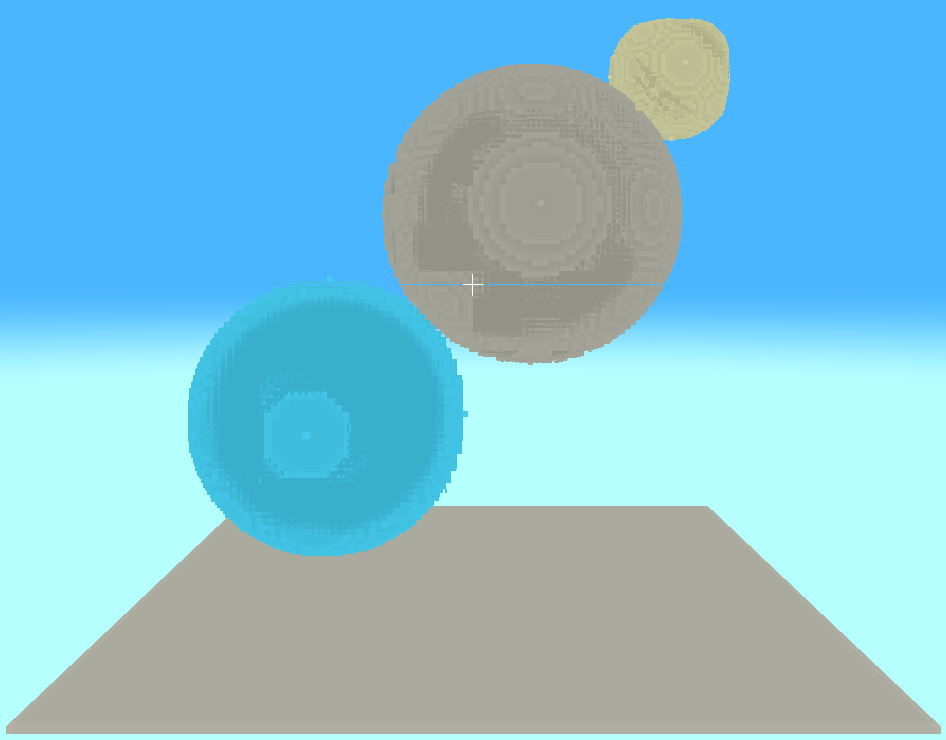
\includegraphics[width=\textwidth]{figures/hybrid_focus_1.png}
        \caption{1x1 focus size at the center of the world.}
    \end{subfigure}
    \hfill
    \begin{subfigure}[t]{0.32\textwidth}
        \centering
        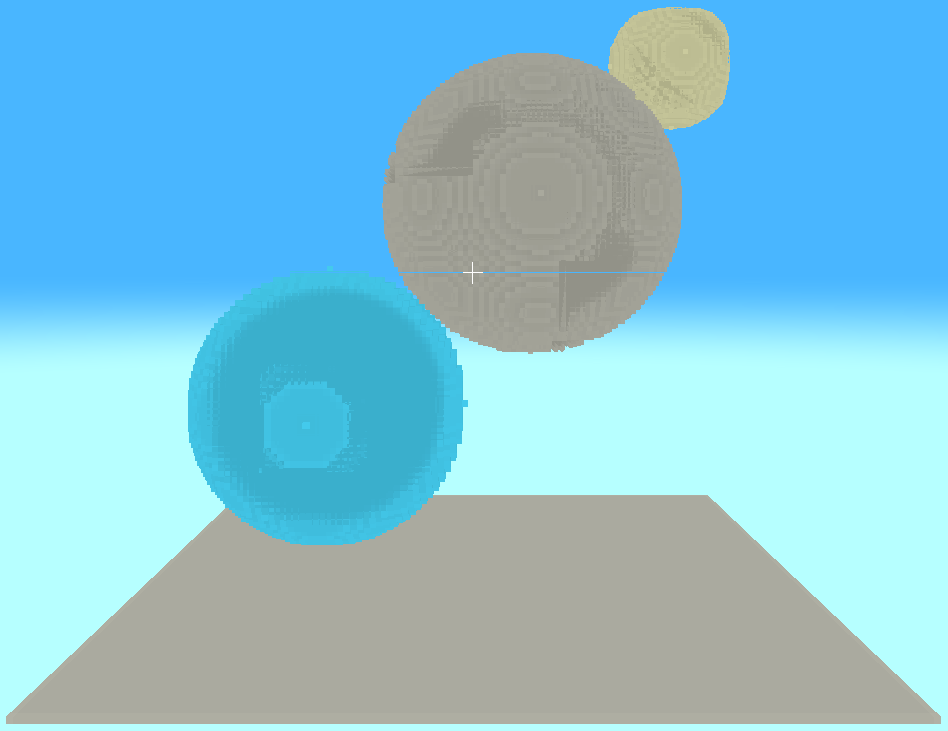
\includegraphics[width=\textwidth]{figures/hybrid_focus_2.png}
        \caption{A 2x2 focus size at the center of the world.}
    \end{subfigure}
    \hfill
    \begin{subfigure}[t]{0.32\textwidth}
        \centering
        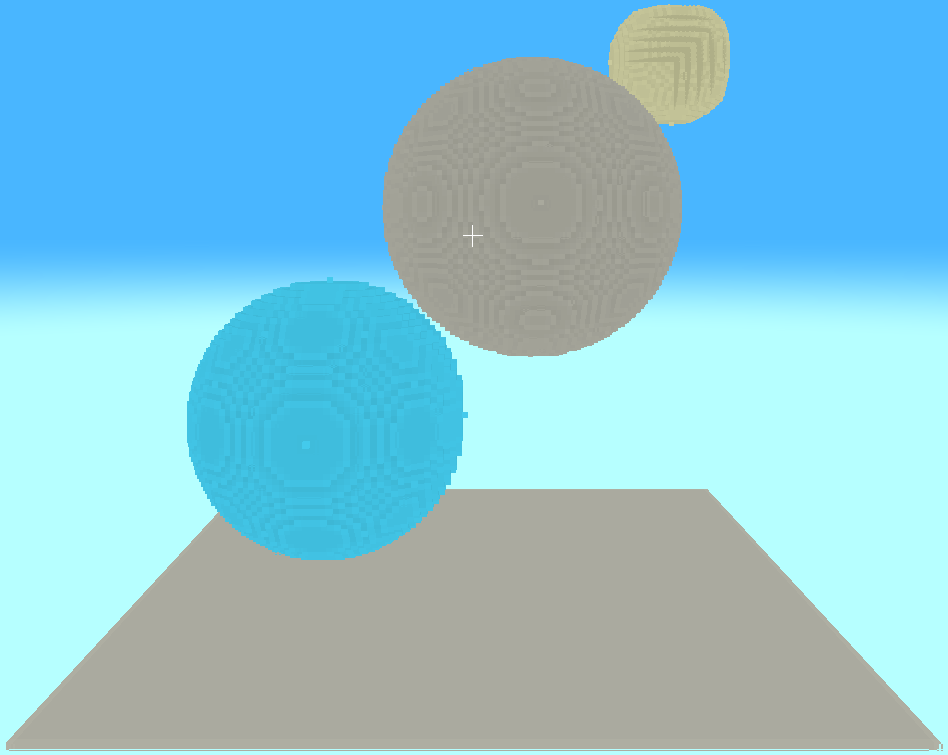
\includegraphics[width=\textwidth]{figures/hybrid_focus_3.png}
        \caption{Focus size encompassing the whole world.}
    \end{subfigure}
    \caption{Comparison of the rendering artifacts and distance values inaccuracies introduced by utilizing JFA in regions
        outside the focus point.}
    \label{fig:focus_size_artifacts}
\end{figure}

\section{Optimized implementation}
This section will focus on applying various optimization to the Algorithm described in Section~\ref{sec:lod_jfa_fim} to
achieve the best possible performance.

\subsection{JFA GPU Synchronization} \label{sec:jfa_gpu}
Section~\ref{sec:jfa} covers the Jump Flooding Algorithm in detail, but the chosen implementation in that section was for
the compute shader to execute a single pass of the algorithm. This approach means that the CPU is required to wait on the
GPU to flag that the required buffers are no longer in use before the next pass, at a smaller step size, can be
dispatched by the CPU.

The CPU uses fences to wait for the GPU to signal when required resources are no longer in use by the GPU, this requires
synchronization across the CPU and GPU and, in our case with large buffers, is an expensive process, especially as the
number of buffers and chunks increases.

An updated algorithm for JFA with the logic for iterating through decreasing step sizes can be seen in
Algorithm~\ref{alg:jfa_opt}; this is implemented in a single compute shader, as such the CPU now only needs to dispatch
the compute shader once with an initial step size, and the required number of iterations.

\begin{algorithm}[H]
    \caption{Jump Flooding Algorithm with Iterations}
    \label{alg:jfa_opt}
    \begin{algorithmic}[1]
        \REQUIRE Voxel grid size \(N\), Voxel grid \(V\), Voxel location \((x, y, z)\), Initial Step Size \(S_{init}\),
        Required Iterations \(I_{req}\)
        \ENSURE Distance field grid \(D\)
        \STATE \texttt{voxel} $\gets$ \texttt{Get Voxel at} \((x, y, z)\)
        \IF{\texttt{voxel is solid}}
        \STATE \textbf{Return:} \(D\)
        \ENDIF

        \STATE Initialize $i \gets 0$
        \FOR{$i < I_{req}$}
        \STATE Initialize $S_{cur} \gets S_{init} >> i$
        \IF{$S_{cur} == 0$}
        \STATE \textbf{Return:} \(D\)
        \ENDIF

        \STATE Initialize $d_{min} \gets$ distance value of voxel at \((x, y, z)\)
        \FOR{neighbours $n$ of voxel $S$ steps away}
        \STATE \texttt{neighbour} $\gets$ \texttt{Get Voxel at} $n$
        \STATE $d_{n} \gets$ distance value of voxel at $neighbour$
        \STATE $d_{min} \gets \min(d_{min}, d_n + S)$
        \ENDFOR

        \STATE \texttt{Memory barrier to synchronize all warps and threads}
        \STATE $i \gets i + 1$
        \ENDFOR
    \end{algorithmic}
\end{algorithm}

\subsection{FIM GPU Synchronization} \label{sec:fim_gpu}
As described in Section~\ref{sec:fim}, the FIM compute shader was responsible for running a single iteration of the FIM
algorithm; a flag is set at the end of the compute shader to indicate whether any changes were made. The CPU is
responsible for dispatching the FIM compute shader until no changes are made to the distance field. A host-visible
buffer was used which contains a flag indicating whether any changes were made to the distance field, this way the GPU is
able to write to it, and the CPU can read and reset it as needed; this requires further fences and barriers to ensure
CPU and GPU don't try to write to the buffer at the same time.

This can be optimized by having a device-only buffer that the GPU is entirely in control of; this buffer will contain a
modified count, and the GPU can then execute another iteration of FIM if no changes were made. An optimized FIM
algorithm used in the compute shader can be seen in Algorithm~\ref{alg:fim_opt}.

\begin{algorithm}[H]
    \caption{Fast Iterative Method with Iterations}
    \label{alg:fim_opt}
    \begin{algorithmic}[1]
        \REQUIRE Voxel grid size \(N\), Voxel grid \(V\), Voxel location \((x, y, z)\)
        \ENSURE Distance field grid \(D\)
        \STATE \texttt{voxel} $\gets$ \texttt{Get Voxel at} \((x, y, z)\)
        \IF{\texttt{voxel is solid}}
        \STATE \textbf{Return:} \(D\)
        \ENDIF

        \STATE Initialize $i \gets 0$
        \STATE Initialize $i_{max} \gets \max(dimension from N)$
        \STATE Initialize $changes \gets 0$

        \FOR{$i < i_{max}$}
        \STATE Initialize $d_{min} \gets N * 2$

        \FOR{neighbours $n$ of voxel}
        \STATE \texttt{neighbour} $\gets$ \texttt{Get Voxel at} $n$
        \IF{\texttt{neighbour is solid}}
        \STATE $d_n \gets 0$
        \ELSE
        \STATE $d_n \gets$ distance value at $n$
        \ENDIF
        \STATE $d_n \gets d_n + 1$
        \STATE $d_{min} \gets \min(d_{min}, d_n)$
        \ENDFOR

        \IF{$d_{min} <$ current distance of $voxel$}
        \STATE Update $D$ at $(x, y, z)$ to $d_{min}$
        \STATE $changes \gets changes + 1$
        \ENDIF

        \STATE \texttt{Memory barrier to synchronize all warps and threads}

        \IF{$changes == 0$}
        \STATE \textbf{Return:} \(D\)
        \ENDIF

        \STATE $i \gets i + 1$
        \ENDFOR
    \end{algorithmic}
\end{algorithm}

\subsection{Single monolithic compute shader} \label{sec:mono_shader}
In the current implementation of level-of-detail as described in Section~\ref{sec:lod_jfa_fim}, each algorithm is
implemented as its own compute shader that is then dispatched by the CPU as needed. This requires further CPU-GPU
synchronization and the re-binding of various (potentially) large buffers; we can instead create a single monolithic
shader that has all the resources needed for each algorithm bound once, and is then responsible for initializing the
distance field, running JFA, and deciding whether FIM should also be run depending on the focus area. The complete
algorithm for this can be seen in Algorithm~\ref{alg:mono_shader}, where there are algorithms referenced they are
included within the implementation but have been excluded for brevity.

\begin{algorithm}[H]
    \caption{Monolithic Compute Shader}
    \label{alg:mono_shader}
    \begin{algorithmic}[1]
        \REQUIRE Chunk voxel grid \(C_{voxels}\), Chunk position \(C_{pos}\),
        Focus area min \(F_{min}\), Focus area max \(F_{max}\), Voxel location \((x, y, z)\)
        \ENSURE Distance field grid \(D\)

        \STATE \texttt{voxel} $\gets$ \texttt{Get Voxel at} \((x, y, z)\)
        \IF{\texttt{voxel is solid}}
        \STATE \textbf{Return:} \(D\)
        \ENDIF

        \STATE Execute \texttt{Algorithm~\ref{alg:fim_init}} on $C_{voxels}$
        \STATE Execute \texttt{Algorithm~\ref{alg:jfa_opt}} on $C_{voxels}$

        \IF{$C_{pos} >= F_{min}$ and $C_{pos} <= F_{max}$}
        \STATE Execute \texttt{Algorithm~\ref{alg:fim_opt}} on $C_{voxels}$
        \ENDIF
    \end{algorithmic}
\end{algorithm}

\subsubsection{Performance Results}
Applying all the optimizations as described in Sections~\cref{sec:jfa_gpu,sec:fim_gpu,sec:mono_shader}, there is a
noticeable improvement in both FPS and compute shader execution time when using a 4x4 focus size. Compute shader
execution time tends to decrease with larger worlds as more chunks will use JFA which is a faster algorithm and so the
average execution time will be less compared to worlds where the focus size means all chunks get recalculated using FIM;
this can be seed in Figure~\ref{fig:mono_shader_fps} and Figure~\ref{fig:mono_shader_exec}.

FPS decreases significantly at larger world sizes; however, this is due to the large overhead in binding a large amount
of storage buffers required by the ray marcher to be able to check all voxels along a ray. Without focussing on areas
such as memory consumption, and alternative representations, or different approaches for rendering distance fields the
FPS will be difficult to improve at large world sizes.

\begin{figure}
    \centering
    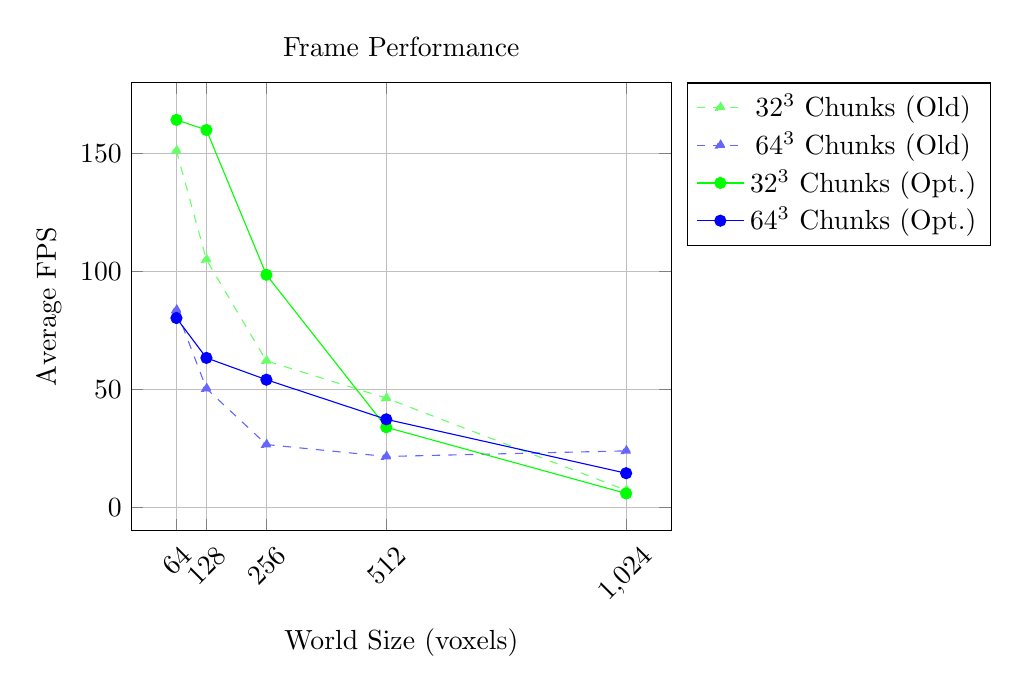
\begin{tikzpicture}
        \begin{axis}[
                title={Frame Performance},
                xlabel={World Size (voxels)}, ylabel={Average FPS},
                xtick={64,128,256,512,1024},
                xticklabel style={rotate=45},
                legend pos=outer north east,
                grid=major
            ]

            \addplot[green!60!white, dashed, mark=triangle*] coordinates {
                    (64,151.27016) (128,105.07455) (256,62.19417) (512,46.41498) (1024,7.3627)
                };
            \addlegendentry{$32^3$ Chunks (Old)}

            \addplot[blue!60!white, dashed, mark=triangle*] coordinates {
                    (64,83.74165) (128,50.44744) (256,26.73361) (512,21.67194) (1024,24.06815)
                };
            \addlegendentry{$64^3$ Chunks (Old)}

            \addplot[green, solid, mark=*] coordinates {
                    (64,164.35240) (128,160.06007) (256,98.68445) (512,34.06396) (1024,6.01326)
                };
            \addlegendentry{$32^3$ Chunks (Opt.)}

            \addplot[blue, solid, mark=*] coordinates {
                    (64,80.36397) (128,63.46359) (256,54.21754) (512,37.43061) (1024,14.58673)
                };
            \addlegendentry{$64^3$ Chunks (Opt.)}
        \end{axis}
    \end{tikzpicture}
    \caption{Comparison of the average FPS of the demo application using the optimized monolithic shader.}
    \label{fig:mono_shader_fps}
\end{figure}

\begin{figure}
    \centering
    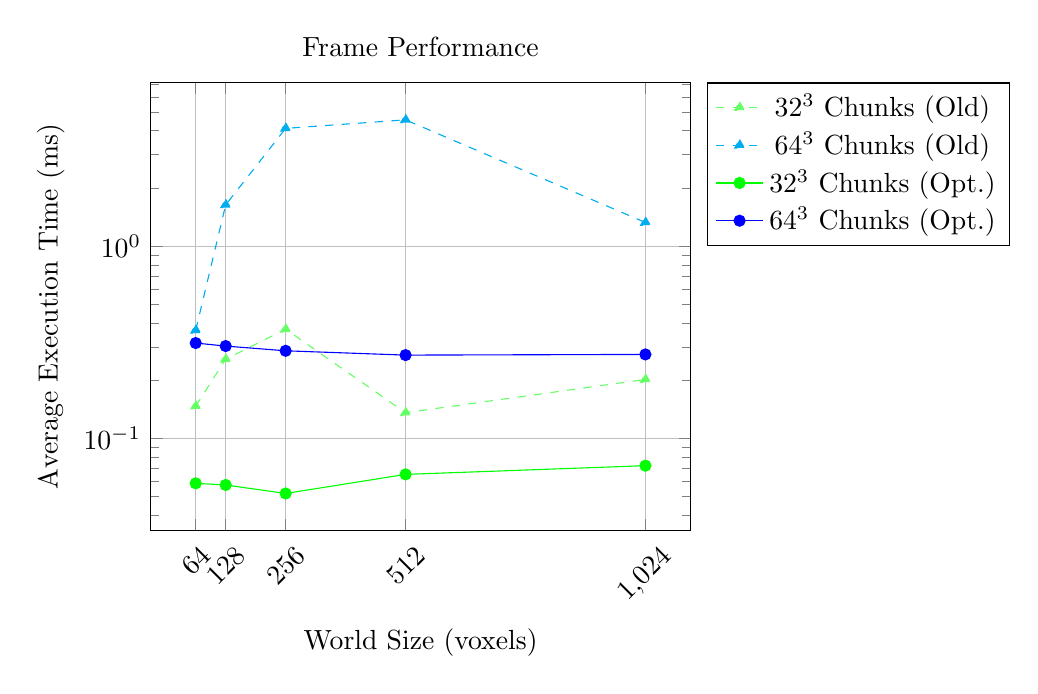
\begin{tikzpicture}
        \begin{axis}[
                title={Frame Performance},
                xlabel={World Size (voxels)}, ylabel={Average Execution Time (ms)},
                xtick={64,128,256,512,1024},
                xticklabel style={rotate=45},
                ymode=log,
                legend pos=outer north east,
                grid=major
            ]

            \addplot[green!60!white, dashed, mark=triangle*] coordinates {
                    (64,0.14759271) (128,0.25882788) (256,0.3710324) (512,0.13646746) (1024,0.20324281)
                };
            \addlegendentry{$32^3$ Chunks (Old)}

            \addplot[cyan, dashed, mark=triangle*] coordinates {
                    (64,0.36615124) (128,1.6450982) (256,4.1130505) (512,4.5542607) (1024,1.3322259)
                };
            \addlegendentry{$64^3$ Chunks (Old)}

            \addplot[green, solid, mark=*] coordinates {
                    (64,0.05855262) (128,0.057403304) (256,0.05185238) (512,0.06516718) (1024,0.07232946)
                };
            \addlegendentry{$32^3$ Chunks (Opt.)}

            \addplot[blue, solid, mark=*] coordinates {
                    (64,0.3142456) (128,0.30305865) (256,0.2863744) (512,0.27198145) (1024,0.27422348)
                };
            \addlegendentry{$64^3$ Chunks (Opt.)}
        \end{axis}
    \end{tikzpicture}
    \caption{Comparison of the average execution time of the optimized monolithic shader.}
    \label{fig:mono_shader_exec}
\end{figure}

\subsection{Pure Distance Field}
As described in Section~\ref{sec:df_repr}, the current distance field encodes colour information as well; this approach
was chosen to reduce the amount of storage buffer objects needed to be bound for the ray marcher. As shown in the
optimized monolithic shader in Section~\ref{sec:mono_shader}, this methodology severely limits the FPS of the
demonstration application at large world sizes. Instead of attempting to optimize the ray marcher to handle a large
amount of distance fields, we can optimize the distance field to only store the distances and have the ray marcher
calculate colours.

This approach is expected to make the FPS of the demonstration application worse; however, reducing the number of bit
operations the distance field compute shader needs to carry out could improve the execution time.

\subsubsection{Performance Results}

